\newpage
\section{Front-end}

As mentioned the requirements, I used React for front-end. The main folder structure can be seen at the appendicies \hyperref[front-end-tree]{front-end-tree}. I used \textbf{antd}, which is an enterprise-class UI design language and React UI library, for user interface, Node.js, which is a JavaScript runtime built on Chrome's V8 JavaScript engine, and npm, packages manager.

In the front-end part, there are 2 main folders: public and src. The folder public contains the default \texttt{public.html} when npm is used to create the project and \texttt{public.html} contains only one div whose id is `\texttt{root}' and which will be modified through entire app. 

\subsection{Folder Structure}

The main project files are inside the src folder.
\begin{itemize}
  \item \texttt{globals}: It is a folder and contains the global variables of the app.
  \item \texttt{pages}: It is a folder and contains the pages, called auth, book, and user, as well as the main homepage of the app.
  \item \texttt{service}: It is a folder and contains the service layer of front-end. Files inside this folder include functions to connect the back-end.
  \item \texttt{App.js}: It is a file and responsible for rendering the pages and providing the main/top navigations around the app. Also, it checks the authorization token and its validation.
  \item \texttt{index.js}: It is a file and responsible for rendering \texttt{App.js} by using \texttt{ReactDOM}.
\end{itemize}

I will briefly explains the folder and files in detail. Then I will tell the pages.

\subsubsection{\texttt{globals}}

This folder contains just a file, called \texttt{GlobalVariables}. That file contains two global variables, called \texttt{BOOK\_COLUMNS} and \texttt{PAGINATION} which are used for tables around app.

\begin{figure}[ht]
  \centering
  \begin{forest}
    pic dir tree,
    where level=0{}{% folder icons by default; override using file for file icons
      directory,
    },
    [\dots
      [globals
        [GlobalVariables.js, file]
      ]
    ]
  \end{forest}
  \caption{Structue of globals}
\end{figure}

\subsubsection{\texttt{pages}}

This folder contains the whole pages, which means users mainly see the files inside this folder. I will explain the pages in details later.

\begin{figure}[ht]
  \centering
  \begin{forest}
    pic dir tree,
    where level=0{}{% folder icons by default; override using file for file icons
      directory,
    },
    [\dots
      [pages
        [auth
          [\dots, file]
        ]
        [book
          [\dots]
        ]
        [user
          [\dots]
        ]
        [Home.js, file]
      ]
    ]
  \end{forest}
  \caption{Structue of pages}
\end{figure}

\paragraph{\texttt{Home.js}:}

This is the homepage of the app and contains the general information of the user. It can be accessed by clicking the \texttt{Home} from the top navigation.

\paragraph{\texttt{auth}:}

This folder contains just a file, called \texttt{Login}, and it is responsible for login page.

\paragraph{\texttt{book}:}

This is the page of books. It contains five folders and one file inside it, and is responsible for the operations adding, deleting, updating and adding/remove books to/from favorite/read lists. It uses switch for rendering the right page of the operaiton.

\paragraph{\texttt{user}:}

This is the page of users. It contains four folders and one file inside it, and is responsible for the operations adding, deleting, updating. It uses switch for rendering the right page of the operaiton.

\subsubsection{\texttt{service}}

This folder contains the services to access the back-end. The functions inside the service files handle the returned response and return new object with the data inside response. Additionally, thanks to axios interceptor, authorization token, which is saved to \texttt{Session Storage} or \texttt{Local Storage} while logging in, is added the header of all requests.

\begin{figure}[ht]
  \centering
  \begin{forest}
    pic dir tree,
    where level=0{}{% folder icons by default; override using file for file icons
      directory,
    },
    [\dots
      [service
        [AuthService.js, file]
        [BookListService.js, file]
        [BookService.js, file]
        [UserService.js, file]
      ]
    ]
  \end{forest}
  \caption{Structue of service}
\end{figure}

\begin{itemize}
  \item \texttt{AuthService}: Responsible for authentication and login process.
  \item \texttt{BookListService}: Responsible for adding/removing books to/from read/favorite lists.
  \item \texttt{BookService}: Responsible for book operations such as searching, adding, removing and updating.
  \item \texttt{UserService}: Responsible for user operations such as searching, adding, removing and updating.
\end{itemize}

\subsection{Pages}

When the app is run, firstly \texttt{index.js} renders the \texttt{App.js}. \texttt{App.js} firstly checks the authorization token and its validation. If the token is valid, it directs user to the homepage, rendering (\texttt{Home.js}). If the token is not valid, it directs user to the login page, rendering (\texttt{Login.js}).

\subsection{Login and Logout}

This page contains basic login form. While login page is done by antd form, logout item is constructed by `Popconfirm' of antd. If the `\texttt{Remember me}' option is chosen, auhorization token is saved into both \texttt{Session Storage} and \texttt{Local Storage}. However, if it is not chosen, the token is only saved into \texttt{Session Storage}.

\begin{minipage}{.49\textwidth}  
  \begin{figure}[H]
    \centering
  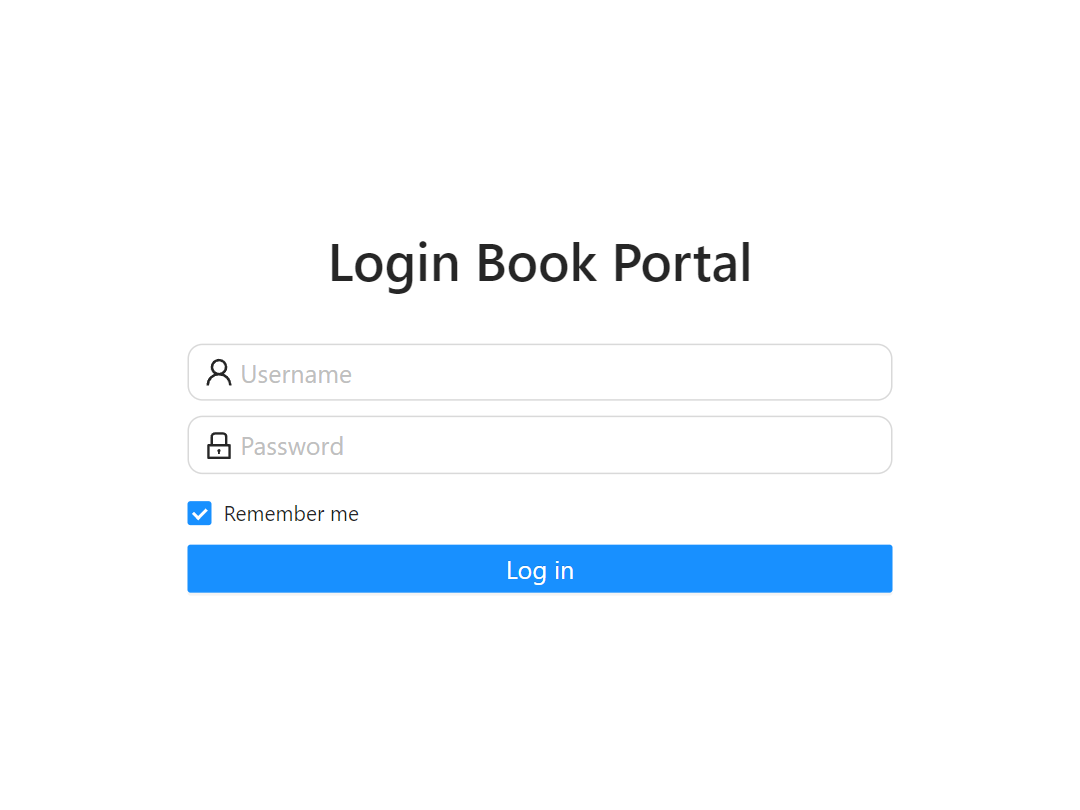
\includegraphics[width=\textwidth]{img/front-end/login-page.png}
  \caption{Login Page}
  \end{figure}
\end{minipage}
\begin{minipage}{.49\textwidth}
  \begin{figure}[H]
    \centering
  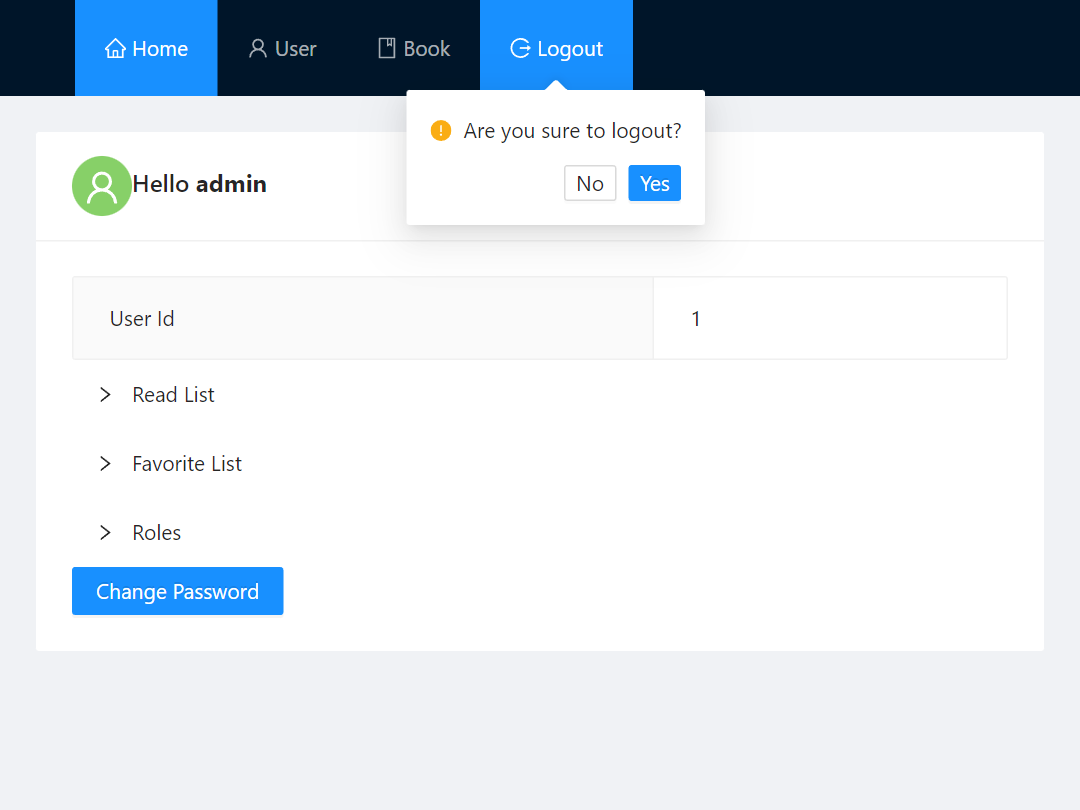
\includegraphics[width=\textwidth]{img/front-end/logout.png}
  \caption{Logout}
  \end{figure}
\end{minipage}

% \begin{figure}[ht]
%   \centering
%   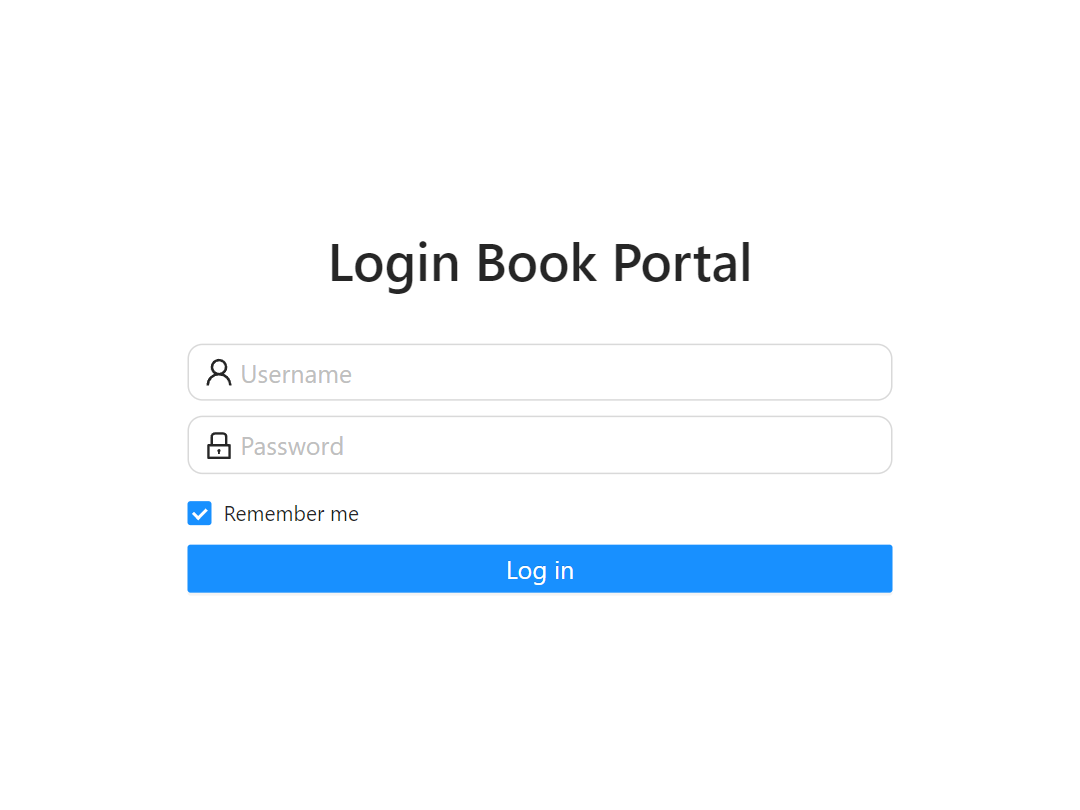
\includegraphics[width=\textwidth]{img/front-end/login-page.png}
%   \caption{Login Page}
% \end{figure}

After logging in, users are directed to homepage. At the top of the screen, there are four different menu items, called \texttt{Home}, \texttt{User}, \texttt{Book} and \texttt{Logout}. Home is firstly rendering and by using these navigations page can be changed. When users clicked to \texttt{Logout}, a warning, which asks users whether they are sure to logout, popped up that. If yes is clicked, users are directed to login page.

% \begin{figure}[ht]
%   \centering
%   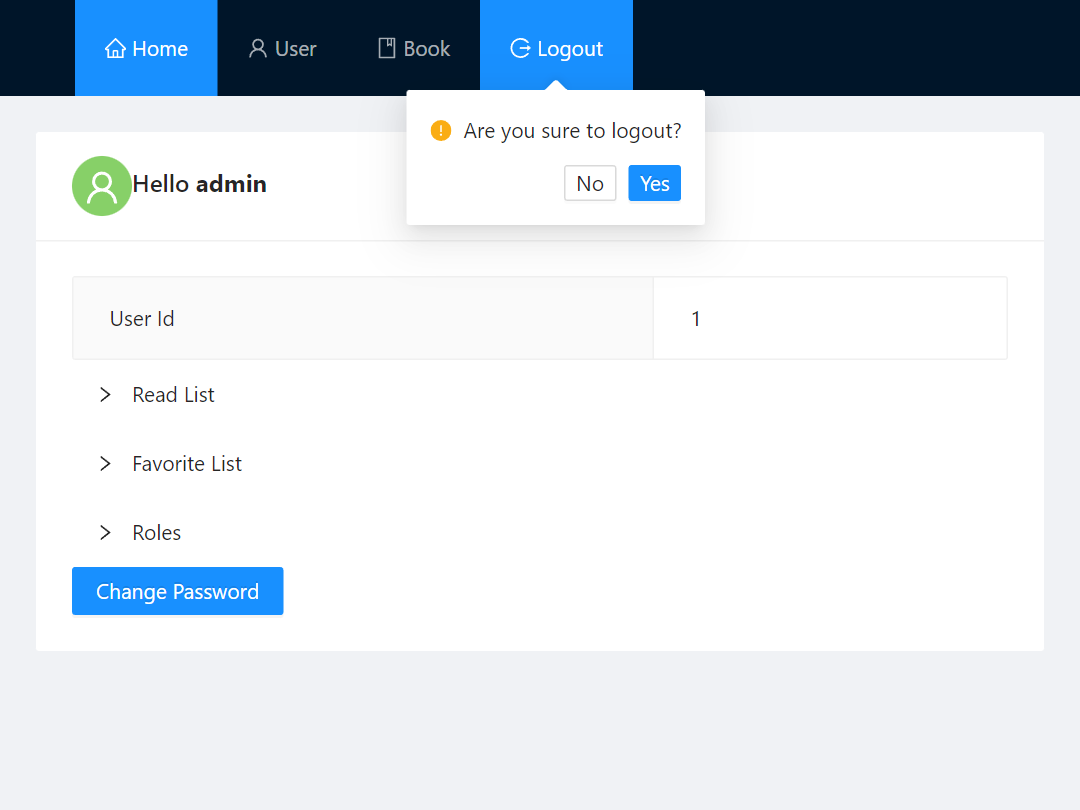
\includegraphics[width=\textwidth]{img/front-end/logout.png}
%   \caption{Logout}
% \end{figure}

\subsection{Home}

In the homepage, user information is provided. This page makes use of `Card', `Descriptions', `Collapse', and `Panel' of antd to show the information. Users can see their user ids, read lists, favorite lists, and roles in this screen. These information is acqiured by sending back-end a request by username and setting information state. By using the button ``Change Password'', they can also access update form and change their passwords.

\begin{minipage}{.49\textwidth}  
  \begin{figure}[H]
    \centering
    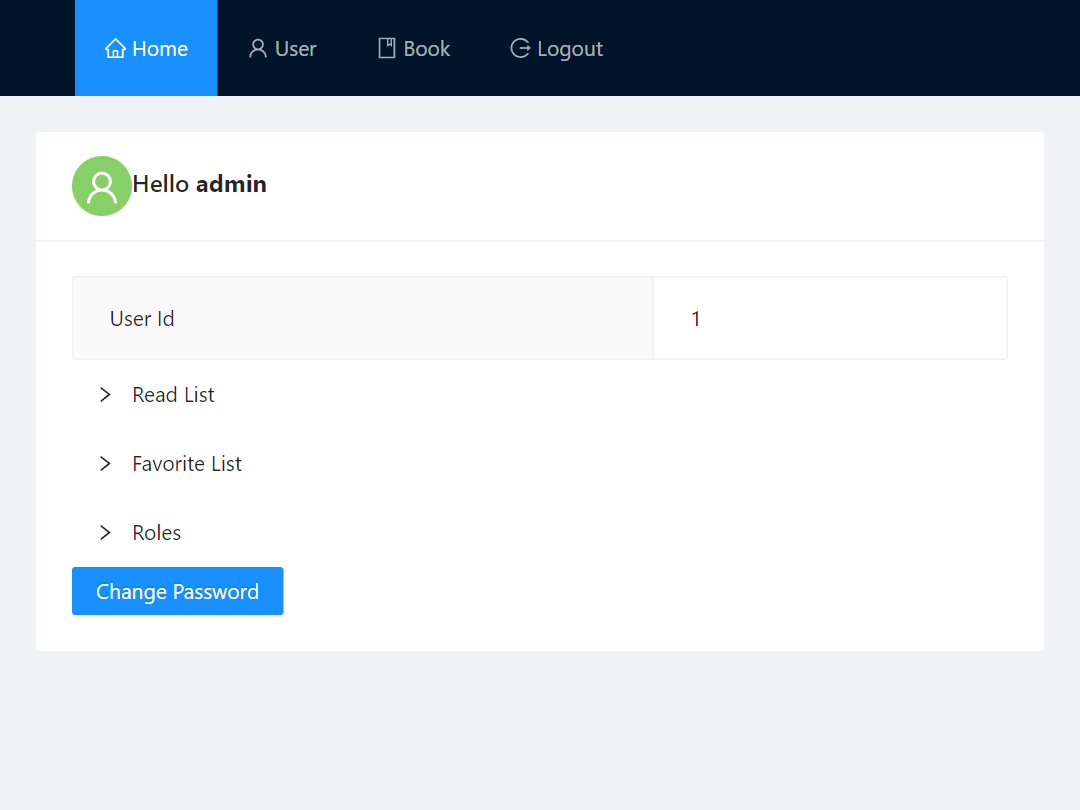
\includegraphics[width=\linewidth]{img/front-end/homepage.png}
    \caption{Home Page}
  \end{figure}
\end{minipage}
\begin{minipage}{.49\textwidth}
  \begin{figure}[H]
    \centering
    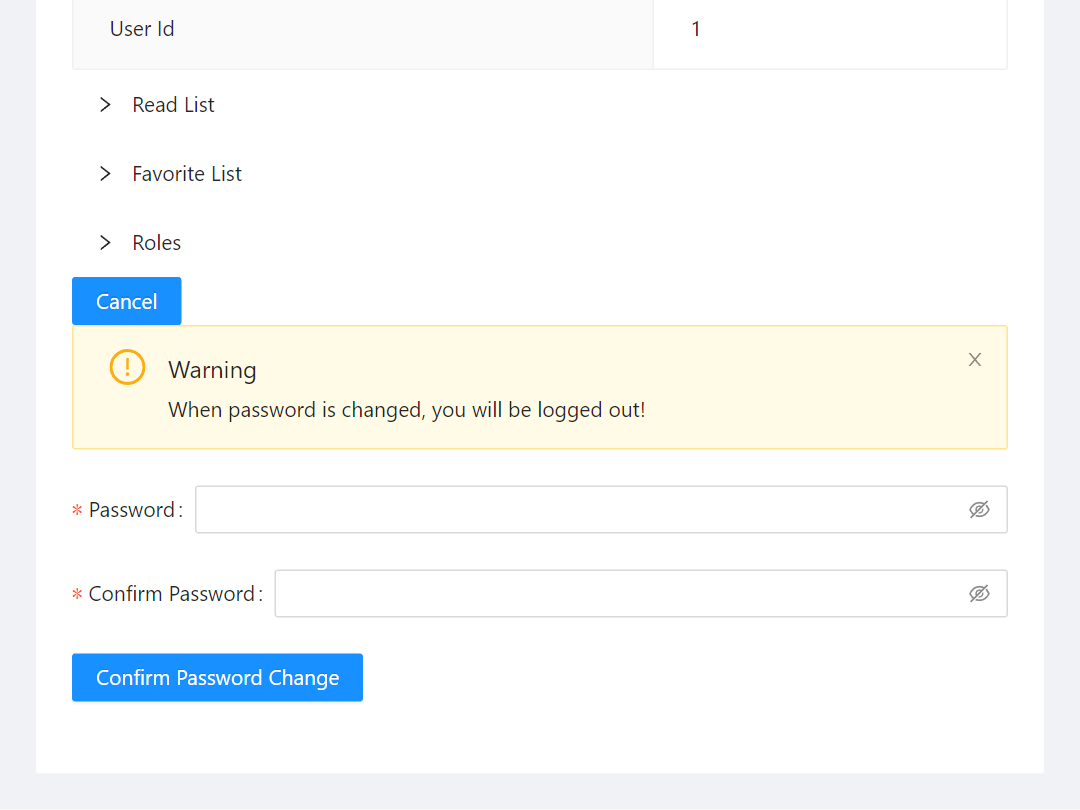
\includegraphics[width=\textwidth]{img/front-end/homepage-password.png}
    \caption{Password Change}
  \end{figure}
\end{minipage}

Since normal users are not allowed to do user operations such as adding, deleting, or updating, \texttt{User} page is special to admins. Therefore, \texttt{User} item is not seen when the user does not have admin roles.

\begin{figure}[H]
  \centering
  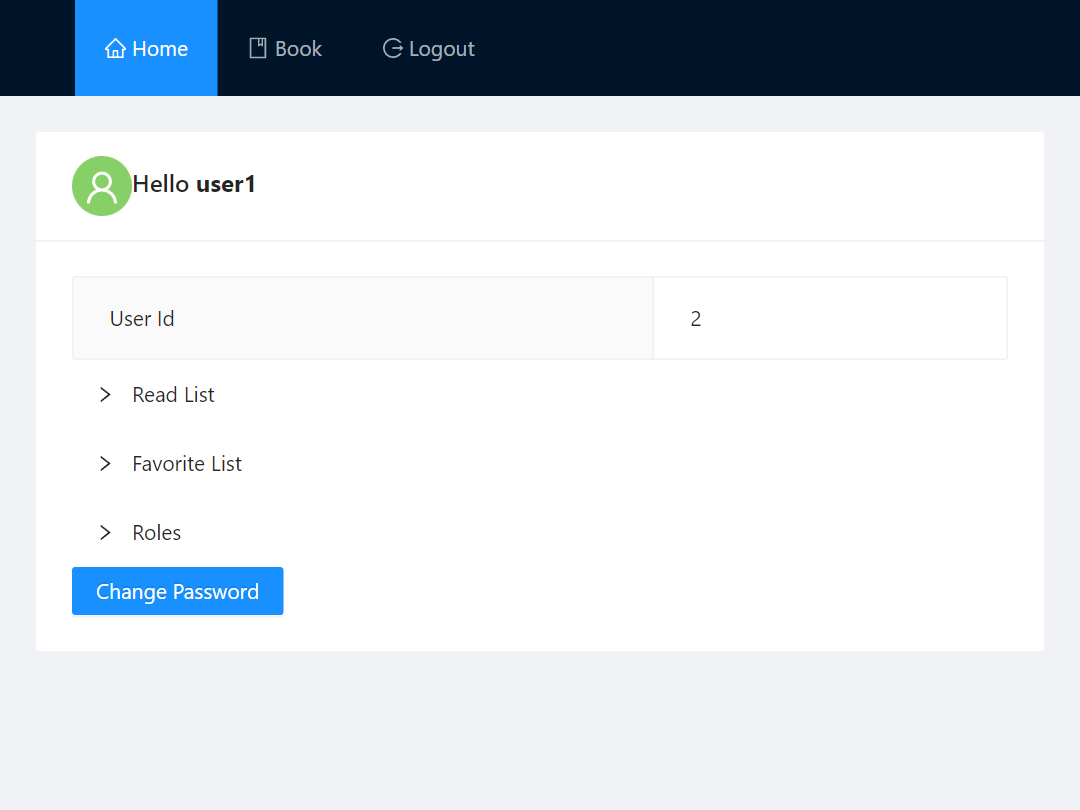
\includegraphics[width=\textwidth]{img/front-end/homepage-user.png}
  \caption{User Home Page}
\end{figure}


\subsection{User}

When \texttt{User} is clicked form top navigaiton, \texttt{User} page is rendered. In this page there are three operations: adding, deleting and updating users. By default \texttt{Add User} is rendered. This page is special to admins because users are not allowed to add, delete, or update users. Therefore, this page is only accessible when the user does not have admin role.

\begin{figure}[H]
  \centering
  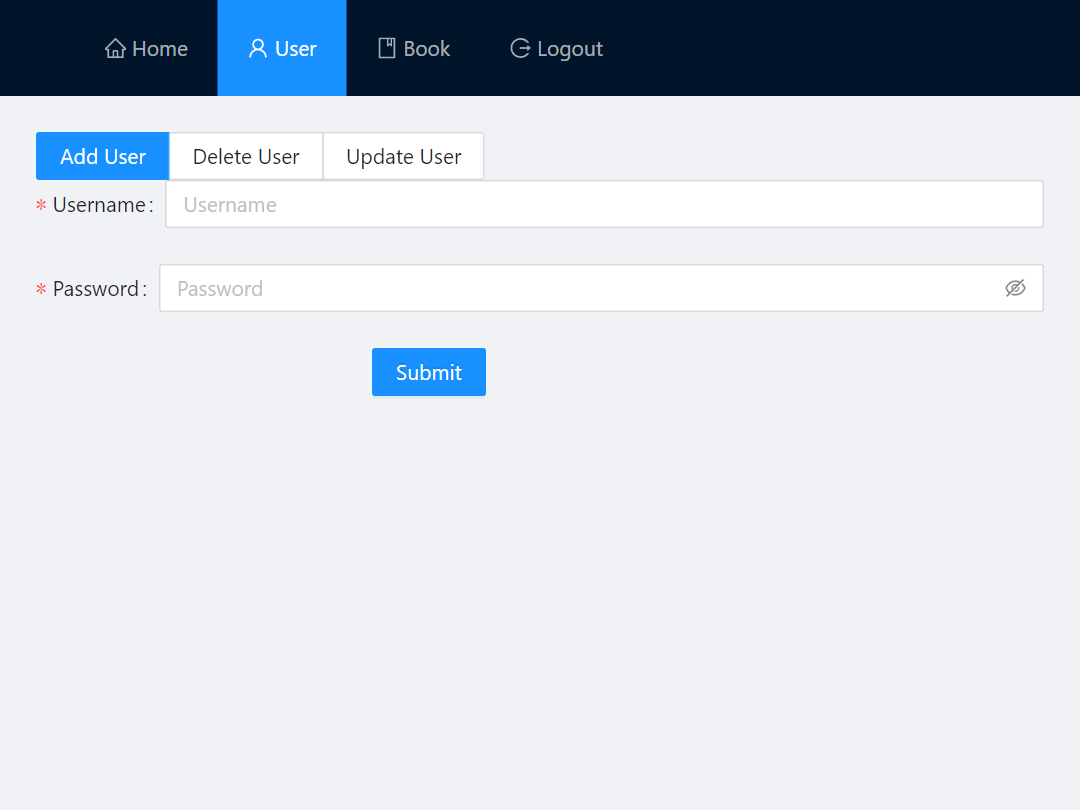
\includegraphics[width=\textwidth]{img/front-end/user.png}
  \caption{User Page}
\end{figure}

\texttt{Add User} contains a basic antd form while \texttt{Delete User} and \texttt{Update User} contains more advanced components. When \texttt{Delete User} and \texttt{Update User} are firstly rendered, a request is sent to database to acquire users and their information by using \texttt{useEffect} of React. These pages also utilize pagination and utilities located in util folder of user.

\texttt{Delete User} and \texttt{Update User} are pretty similar to each other. Both pages support searching users by both id and username, and searching option can be changed by using the radio buttons. When id or username is provided and clicked the search button, a request is sent to back-end through \texttt{UserService}. When the input area is cleared, page is updated and user data is resetted. Both pages also support the pagination and pagination setting changes. Admin can change the pagination setting by using the navigation below. When pagination is changed, a new request is sent to back-end. Additionally, in both pages, admin can see the information of the users.

\begin{minipage}{.49\textwidth}
  \begin{figure}[H]
    \centering
    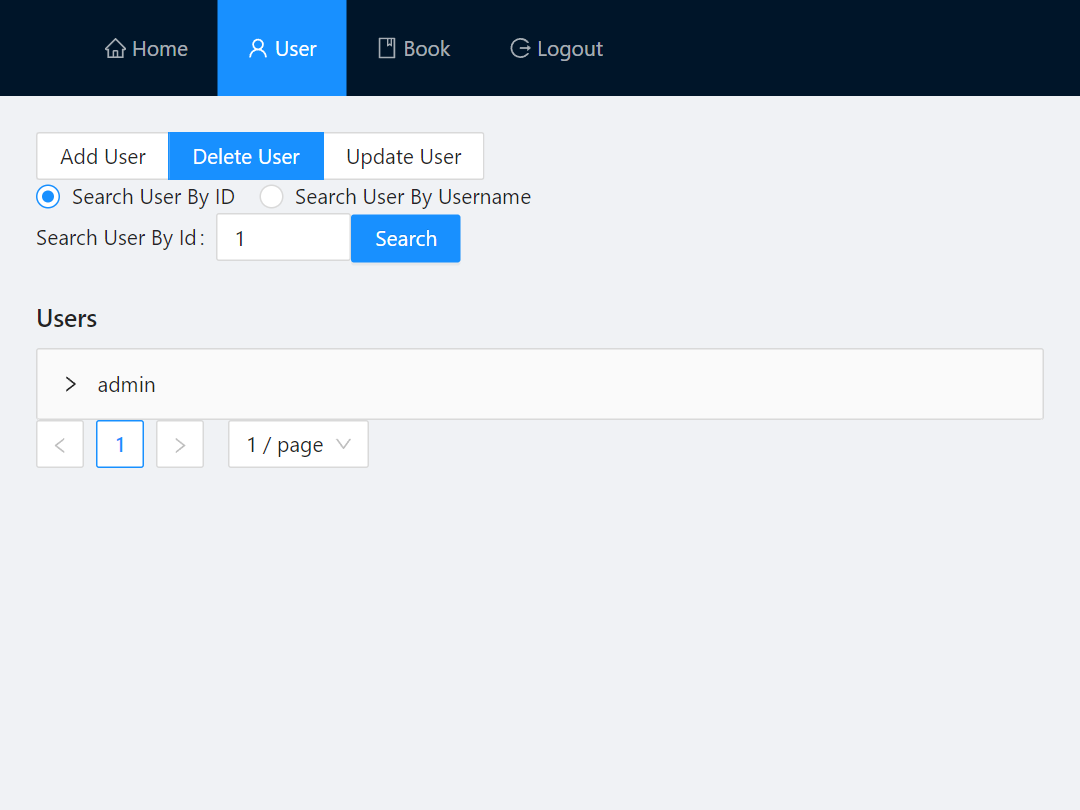
\includegraphics[width=\linewidth]{img/front-end/user-delete-id-search.png}
    \caption{Searching by ID}
  \end{figure}
\end{minipage}
\begin{minipage}{.49\textwidth}
  \begin{figure}[H]
    \centering
    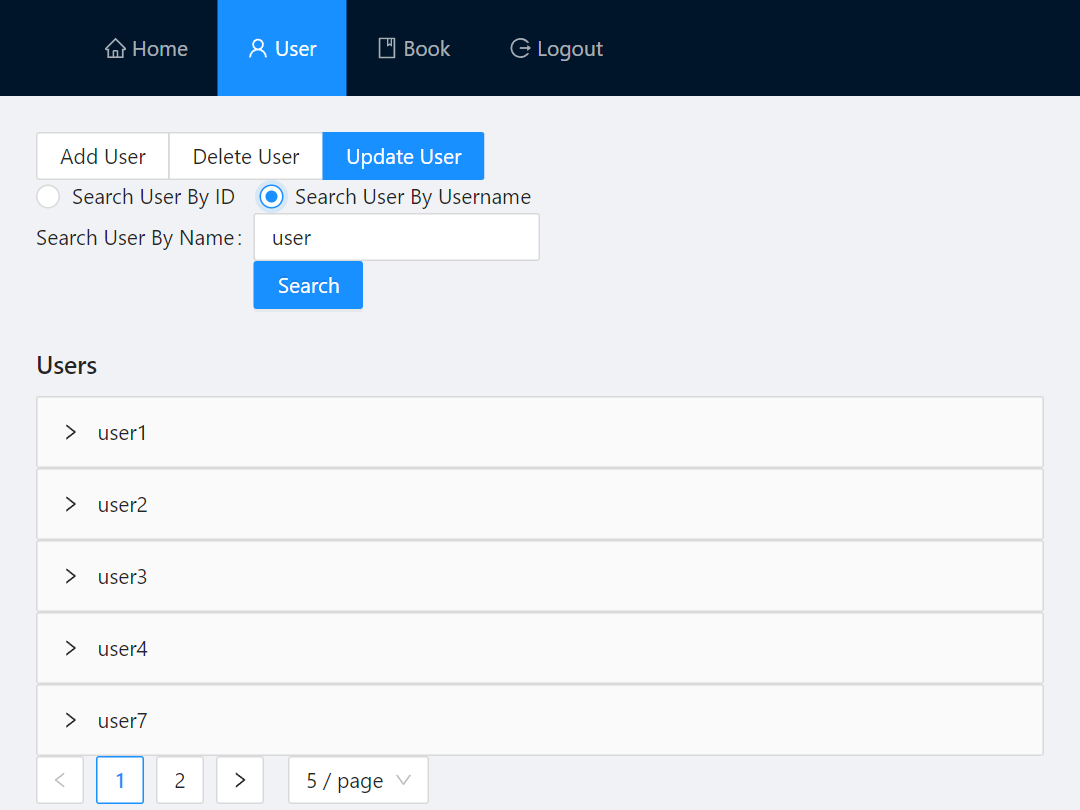
\includegraphics[width=\linewidth]{img/front-end/user-update-name-search.png}
    \caption{Searching by Name}
  \end{figure}
\end{minipage}

Pagination and visualizing the data was the most hard part for me because there were several aspects I need to consider. I changed my visualizing method third times for convenience of developing. Because of this reason, I had to change back-end at some points, so I lost so much time for visualizing decision. However, after visualizing decision is done, my job is not done because pagination is a little bit harder than I expected. Since I misunderstood some parts and concepts of pagination and its callback functions, I had to spent a couple of hours to search and read the antd documentation. In the end, I understood what I should do.

The difference between \texttt{Delete User} and \texttt{Update User} is the buttons found in all users. In \texttt{Delete User}, name of button is `Delete User' and it is used for deleting the user. In \texttt{Update User}, name of button is `Update User' and when it is clicked password update form is appeared.

\begin{minipage}{.49\textwidth}
  \begin{figure}[H]
    \centering
    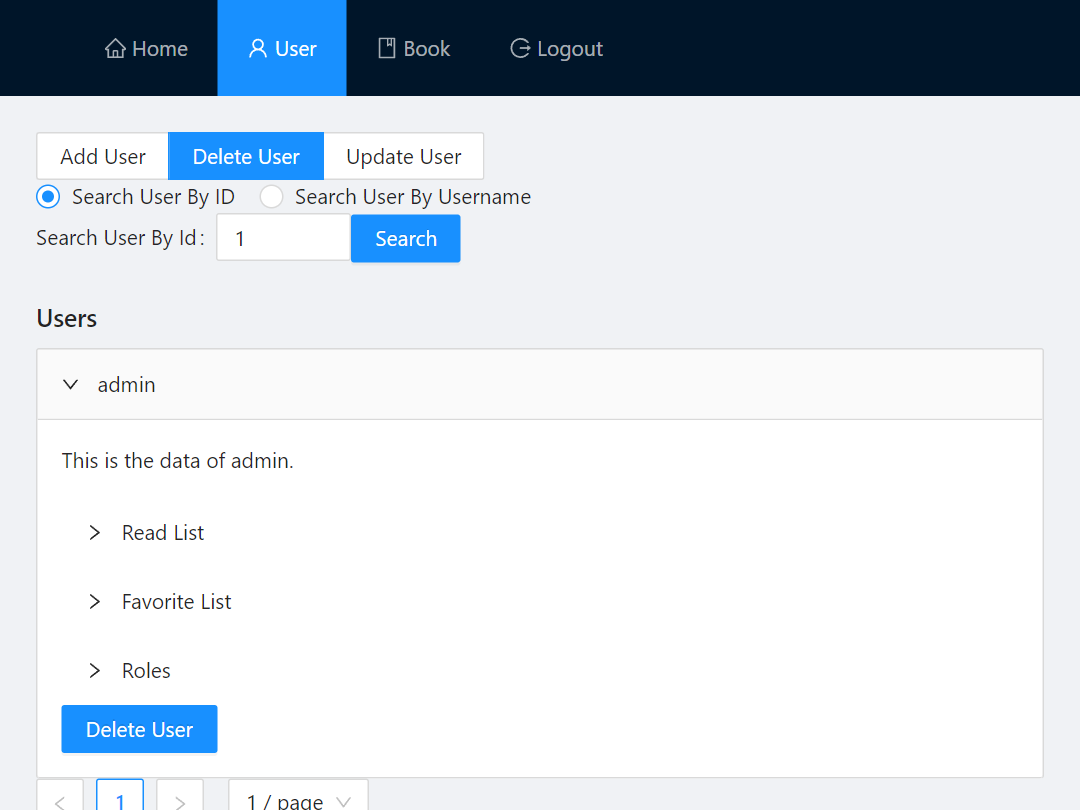
\includegraphics[width=\linewidth]{img/front-end/user-delete.png}
    \caption{Delete User}
  \end{figure}
\end{minipage}
\begin{minipage}{.49\textwidth}
  \begin{figure}[H]
    \centering
    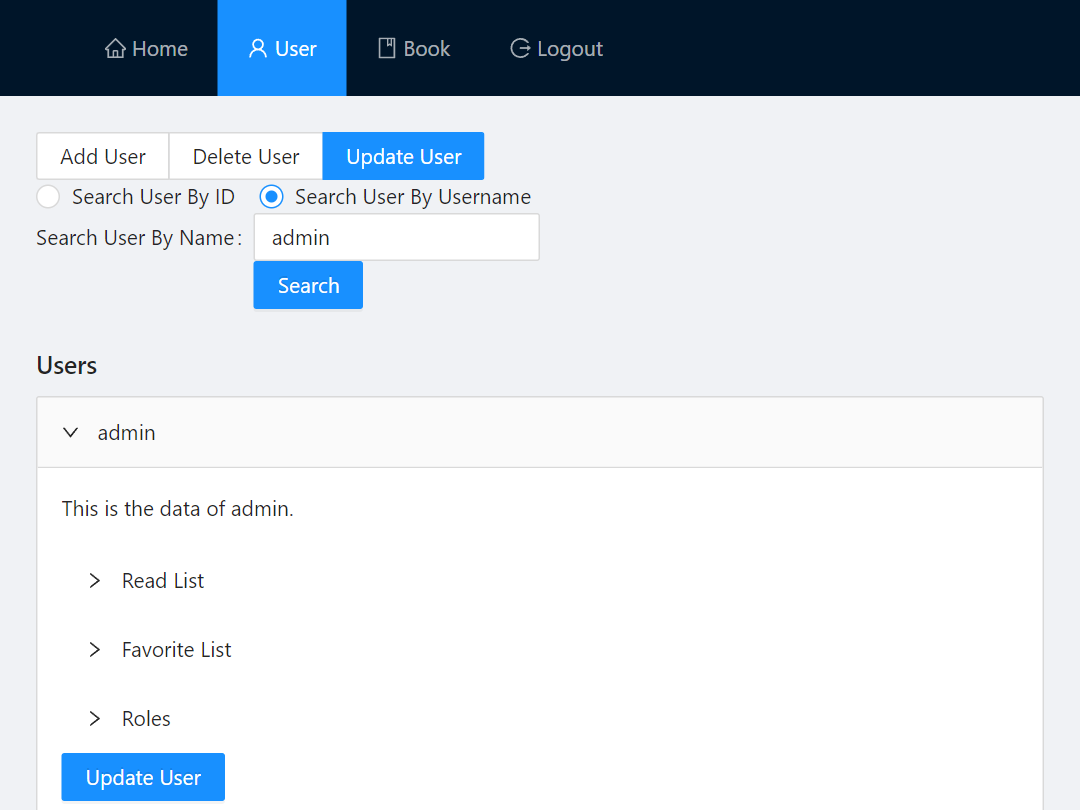
\includegraphics[width=\linewidth]{img/front-end/user-update.png}
    \caption{Update User}
  \end{figure}
\end{minipage}

\subsection{Book}

When \texttt{Book} is clicked form top navigaiton, \texttt{Book} page is rendered. In this page there are three operations: adding, deleting, updating, and listing books. By default \texttt{Book List} is rendered. Although this page is not special, some operations are not allowed to normal users. Therefore; normal users are just allowed listing books and adding/removing these books to/from their lists.

\begin{minipage}{.49\textwidth}
  \begin{figure}[H]
    \centering
    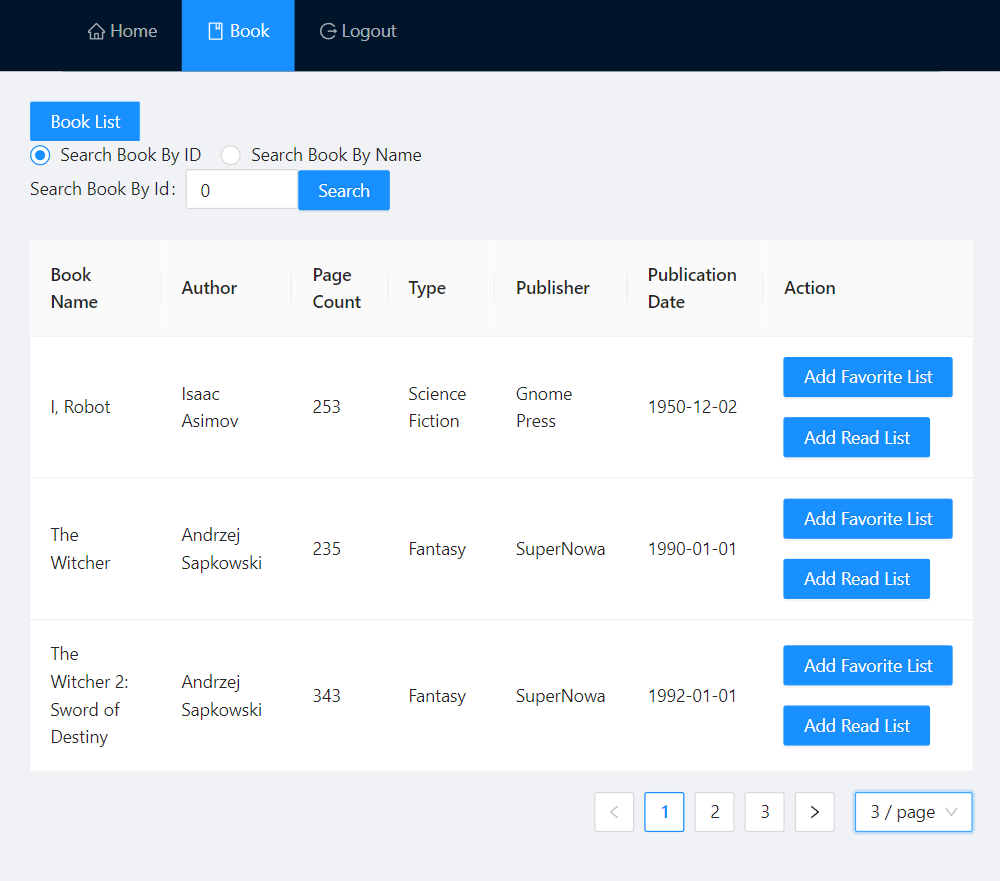
\includegraphics[width=\linewidth]{img/front-end/book-no-admin.png}
    \caption{Book Page for Normal User}
  \end{figure}
\end{minipage}
\begin{minipage}{.49\textwidth}
  \begin{figure}[H]
    \centering
    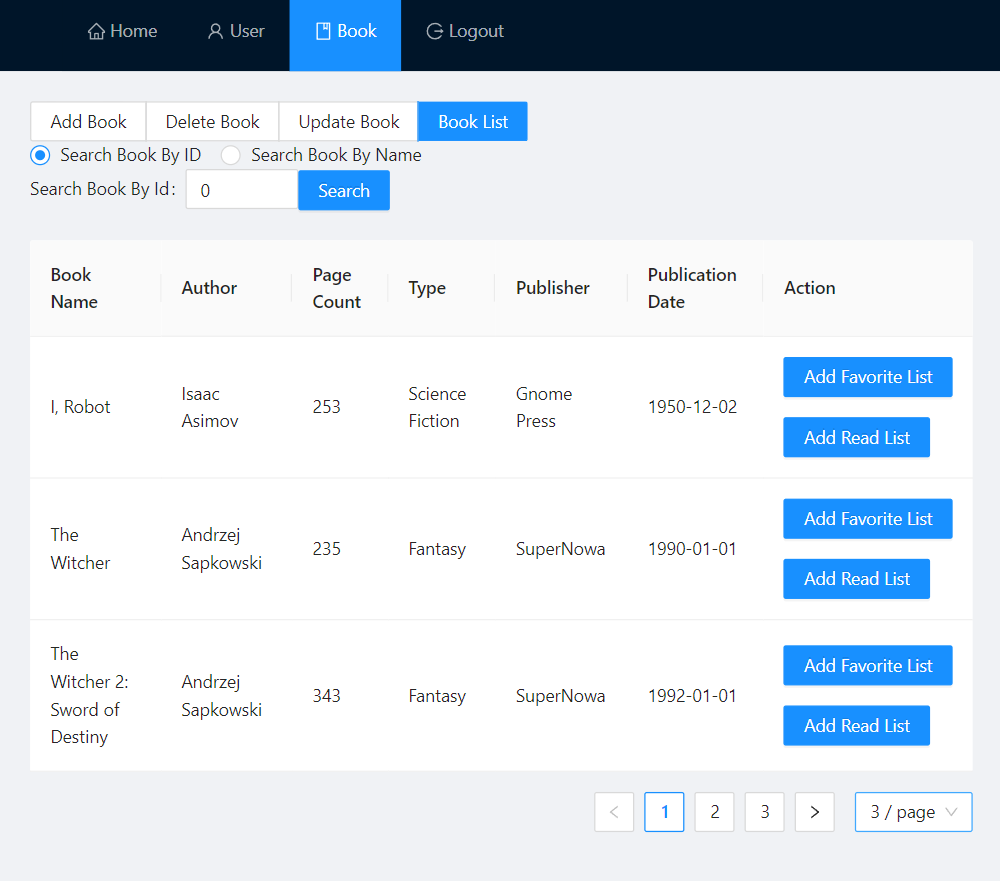
\includegraphics[width=\linewidth]{img/front-end/book-admin.png}
    \caption{Book Page for Admins}
  \end{figure}
\end{minipage}

\subsubsection{\texttt{Add Book}}

This page is for adding book to database and special to admins. When the option is chosen, \texttt{Add Book} is rendered and provides a form to add book. The fields of \texttt{Book} entity: name, author, page count, type, publisher and publication date. All the fields are required and the date can be chosen from calendar. When the book is submitted, a request is sent to back-end to save the book by the help of \texttt{BookService}. When book is saved, the information of the saved book is shown below of the form. Additionally, the size of the form can be changed by using the `Form Size' radio buttons.

\begin{minipage}{.49\textwidth}
  \begin{figure}[H]
    \centering
    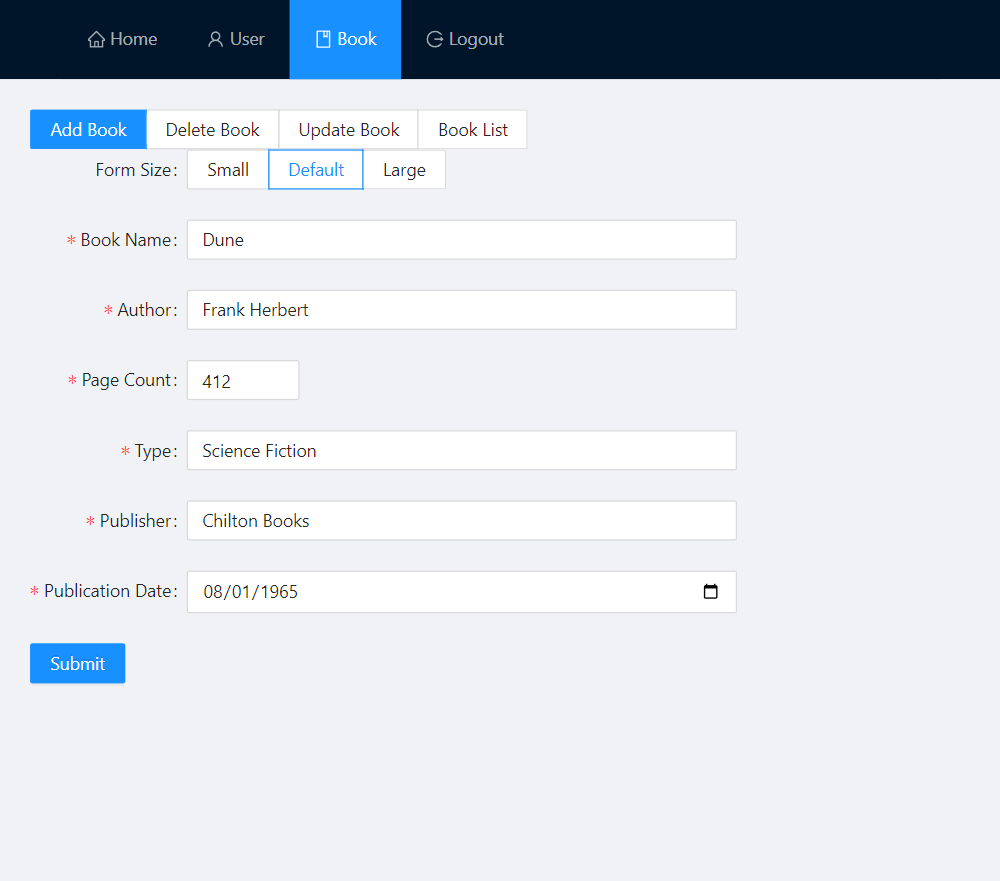
\includegraphics[width=\linewidth]{img/front-end/add-book-form.png}
    \caption{Book Adding Form}
  \end{figure}
\end{minipage}
\begin{minipage}{.49\textwidth}
  \begin{figure}[H]
    \centering
    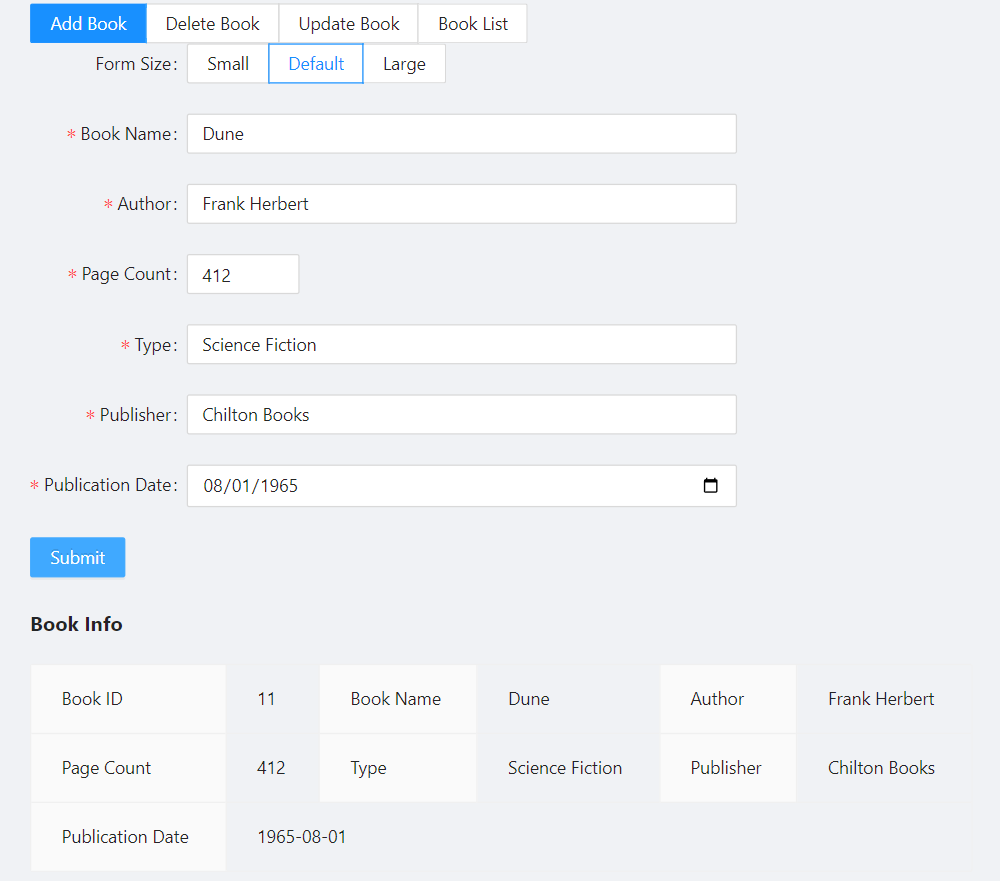
\includegraphics[width=\linewidth]{img/front-end/add-book-added.png}
    \caption{Book Added to Database}
  \end{figure}
\end{minipage}

\subsection{\texttt{Delete and Update Book}}

The \texttt{Delete} and \texttt{Update} pages of the book are similar to user's and special to admins. Both pages support searching books by both id and username, and searching option can be changed by using the radio buttons. Again, when the input area is cleared, page is updated and user data is resetted. Both pages also support the pagination and pagination setting changes. Admin can change the pagination setting by using the navigation below. Additionally, in both pages, admin can see the information of the books.

The only difference between \texttt{Delete Book} and \texttt{Delete User} is the visualizing data. I preffered the `Descriptions' of antd to visualize the data of a book. The differences between \texttt{Update Book} and \texttt{Update User} are the visualizing method and updating form. Only page count, publisher, or publication date of a book can be updated.

\begin{minipage}{.49\textwidth}
  \begin{figure}[H]
    \centering
    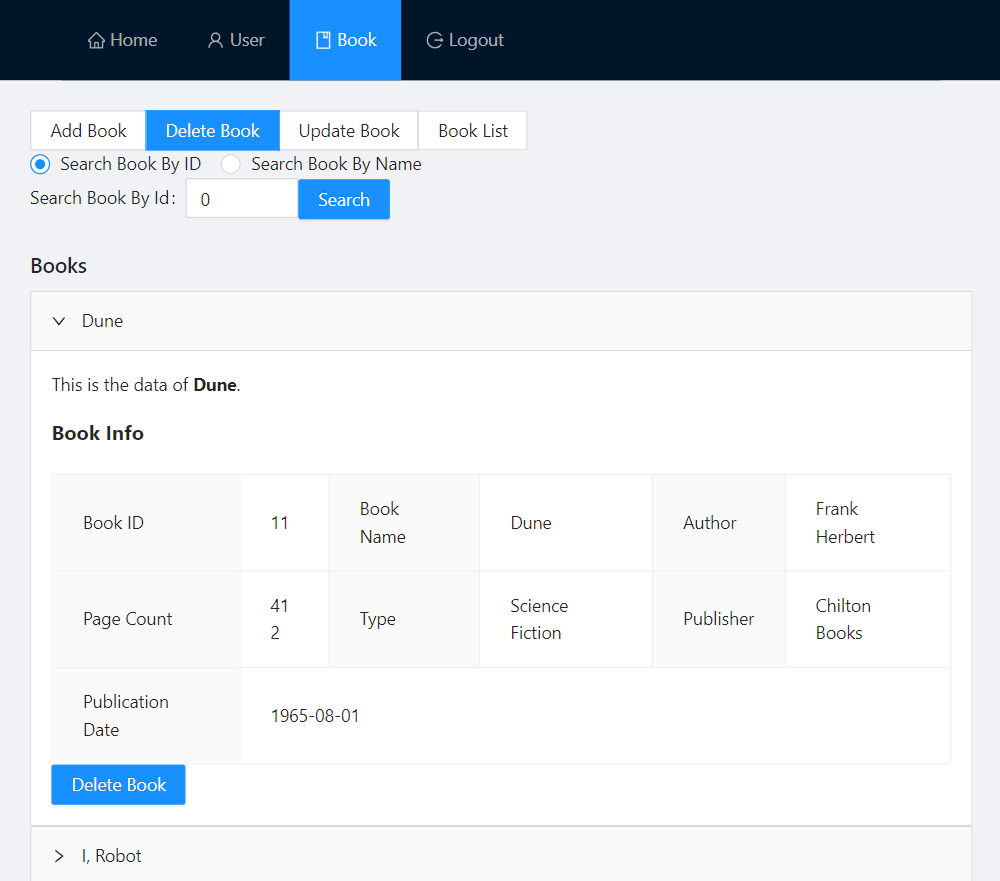
\includegraphics[width=\linewidth]{img/front-end/book-delete.png}
    \caption{Book Delete}
  \end{figure}
\end{minipage}
\begin{minipage}{.49\textwidth}
  \begin{figure}[H]
    \centering
    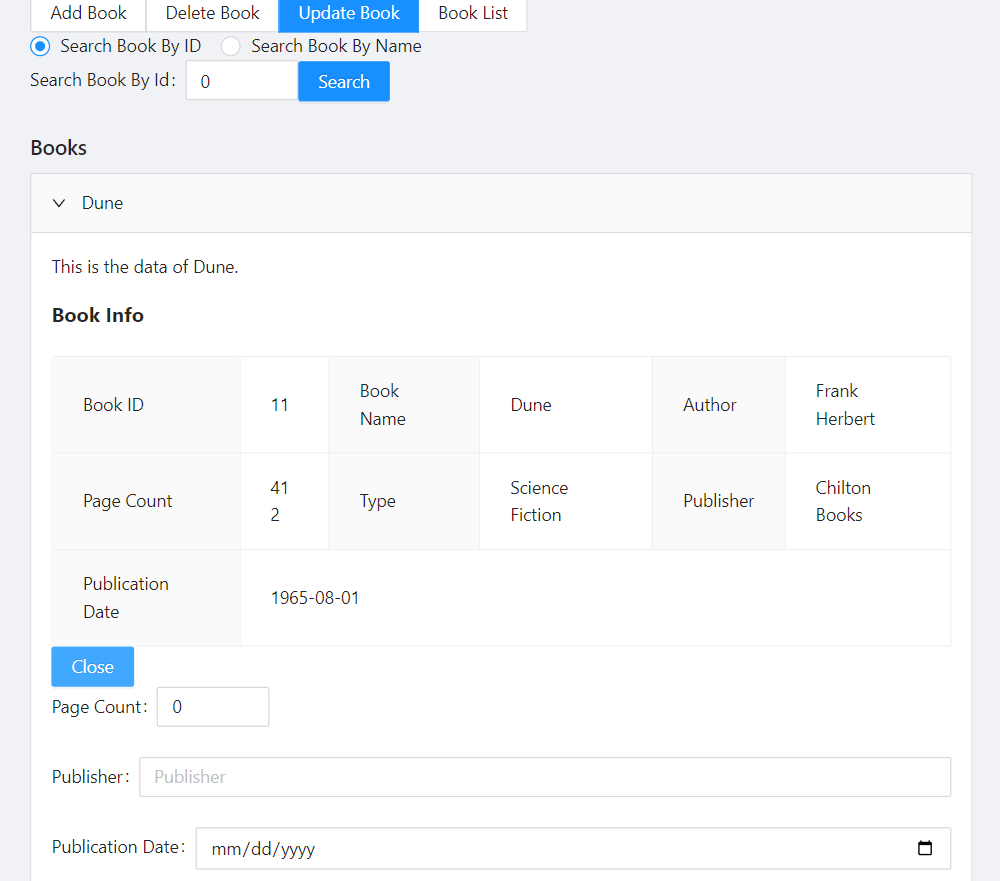
\includegraphics[width=\linewidth]{img/front-end/book-update.png}
    \caption{Book Update}
  \end{figure}
\end{minipage}

\subsection{\texttt{Book List}}

This page is accessible by all users, and the default rendered page of \texttt{Book} item. `Table' and `Pagination' of antd are used in this page and it lists all the books in database and provides searching by both id and name. In each row, information of each book is provided as well as the actions which are operated on the book in that row. Any user can add or remove the book to/from his/her read or favorite lists.

\begin{minipage}{.49\textwidth}
  \begin{figure}[H]
    \centering
    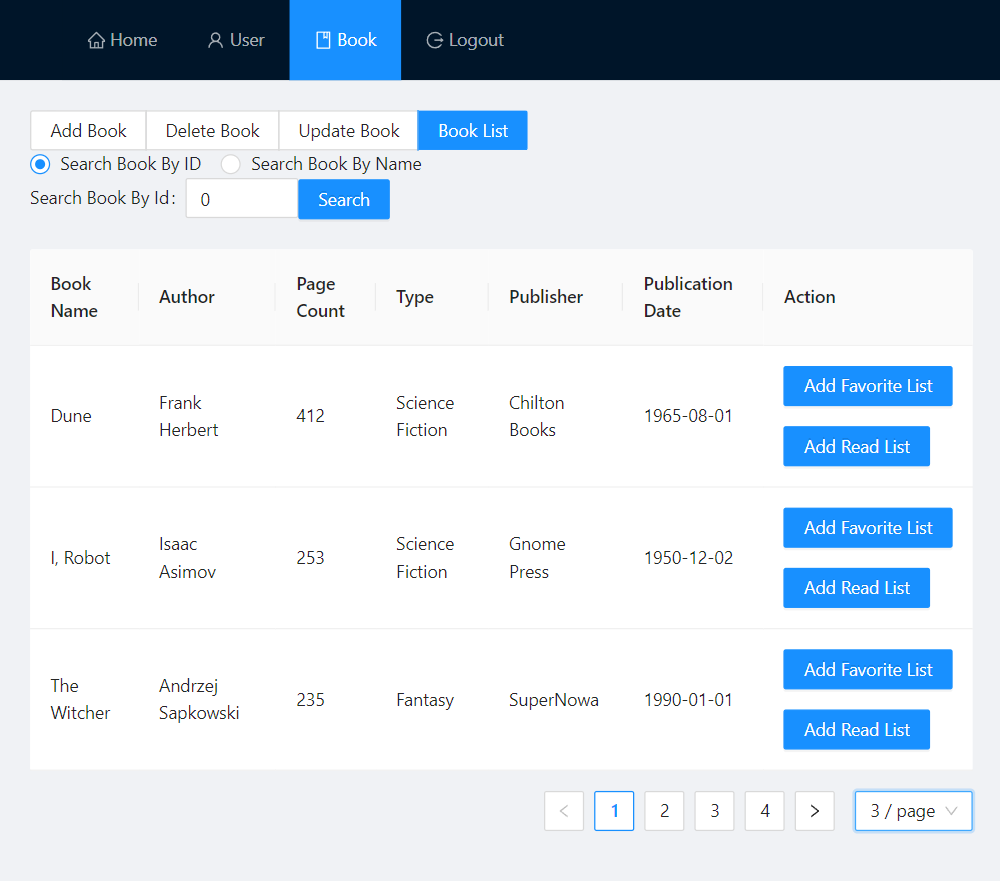
\includegraphics[width=\linewidth]{img/front-end/book-list.png}
    \caption{Book List}
  \end{figure}
\end{minipage}
\begin{minipage}{.49\textwidth}
  \begin{figure}[H]
    \centering
    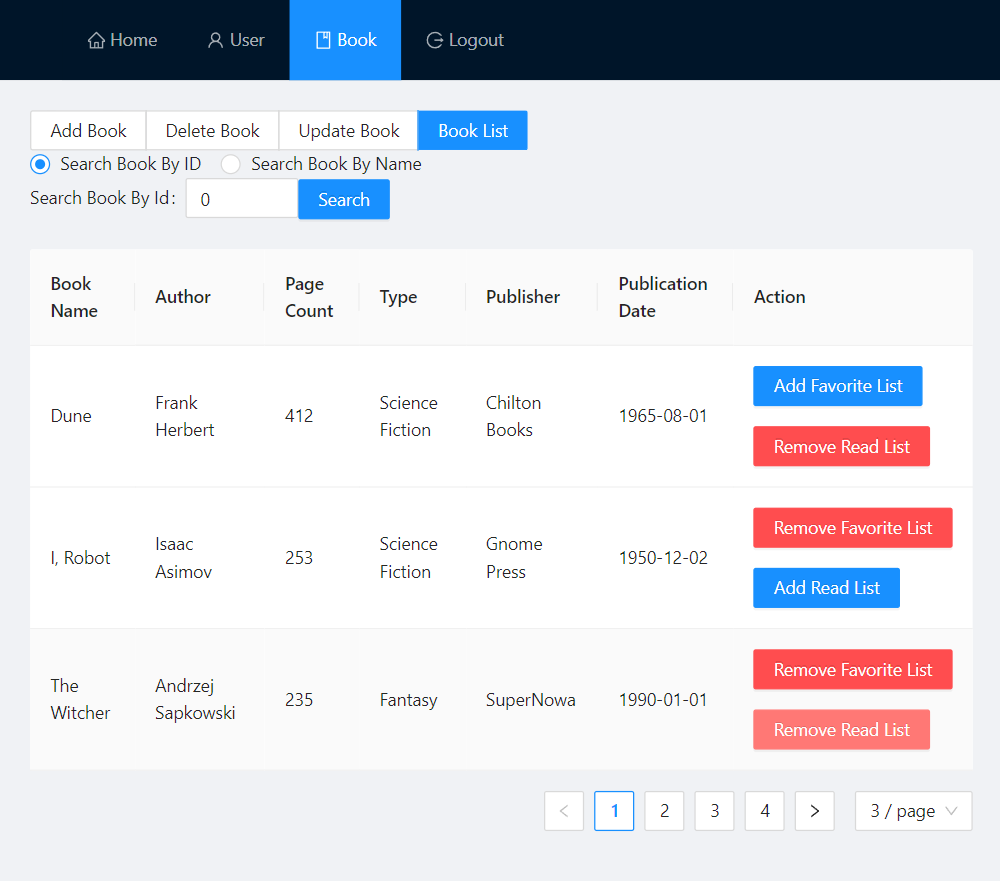
\includegraphics[width=\linewidth]{img/front-end/book-list-example.png}
    \caption{Book List Example}
  \end{figure}
\end{minipage}

If the book is not added to related list, the action button is blue and the text of it specifies the adding operation. However, if the book is already added to related list, the action button is red and the text of it specifies the removing operation. When the button is clicked a request is sent to database and the state of the book data is updated. As a result of that, page is re-rendered with the new state.

This part was hard to code. Putting the action buttons and performing their operations were more difficult, aside from the force of the table. It was easy to send a request and saving the book to user's list at database; however, it was hard to update and re-render the book data and the state of book. I thought to do this task without new getting request because of the complexity. Also, at the first place, the book information had problem when the pagination is updated. To solve these problems, I spent several hours.
